\part{Matematica e teoria}
\chapter{Colori}

\section{Fisica e percezione dei colori}
Il colore che noi percepiamo dipende da due fattori: \textbf{fisico} e \textbf{}.
L'aspetto fisico riguarda il come la luce rimbalza sull'oggetto e poi arriva al
nostro occhio. L'aspetto percettivo riguarda il come il nostro occhio elabora la
luce che arriva produce di conseguenza un colore.

\section{Luce come fenomeno ondulatorio}
La luce come fenomeno ondulatorio \`e caratterizzata da due fattori:
\begin{itemize}
	\item \textbf{Ampiezza}: il valore del picco di ogni onda.
	\item \textbf{Lunghezza d'onda}: la distanza tra due picchi consecutivi. Inversamente
	      proporzionale alla lunghezza d'onda \`e la \textbf{frequenza}: pi\`u i picchi sono
	      vicini pi\`u la frequenza \`e alta. La frequenza si pu\`o ottenere con la formula:
	      \[ f = \frac{c}{l} \]
	      dove $c$ \`e la velocit\`a della luce e $l$ \`e la lunghezza d'onda.
\end{itemize}
Lo spettro della luce visibile ha questo range di lunghezze d'onda

\begin{center}
	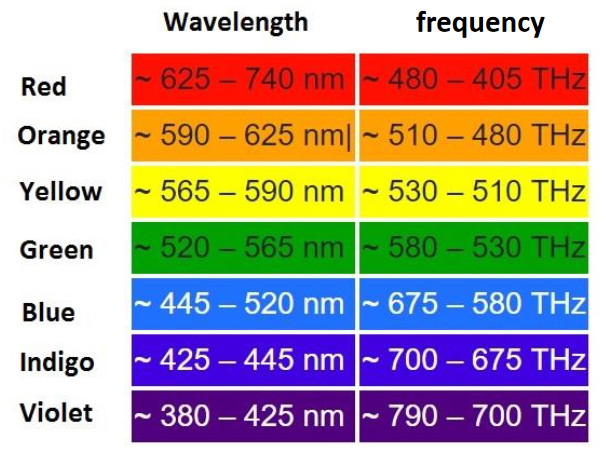
\includegraphics[width=0.5\textwidth]{immagini/spettro_visibile}
\end{center}

\section{Luce come insieme di particelle}
La luce \`e fatta di fotoni, particelle senza massa che viaggiano alla velocit\`a della luce.
Un fascio di luce \`e un insieme di fotoni, ciascuno con la propria frequenza, energia e
colore. Il colore del fascio di luce dipende da come l'insieme di fotoni \`e distribuito sullo
spettro delle frequenze. A noi interessa in particolare questo modo di vedere la luce.

\section{Percezione del colore}
Gli oggetti non hanno un colore, hanno delle propriet\`a fisiche e la luce viene riflessa in
base
\begin{itemize}
	\item alle propriet\`a dei materiali di cui \`e composto l'oggetto.
	\item alle caratteristiche della luce.
	\item al colore intorno all'oggetto.
	\item alla percezione dell'osservatore.
\end{itemize}
La nostra percezione della luce \`e \textbf{additiva}. Se ho quindi due luci di colore diverso
che si sovrappongono vedo la combinazione delle due. Se ho tutti e tre i colori primari insieme
vedo una luce bianca.

Noi vediamo meglio la luce con lunghezza d'onda intorno ai 550nm, ovvero vediamo questi colori
come pi\`u luminosi. La \textbf{funzione di efficienza luminosa fotopica} ce lo mostra.
\begin{center}
	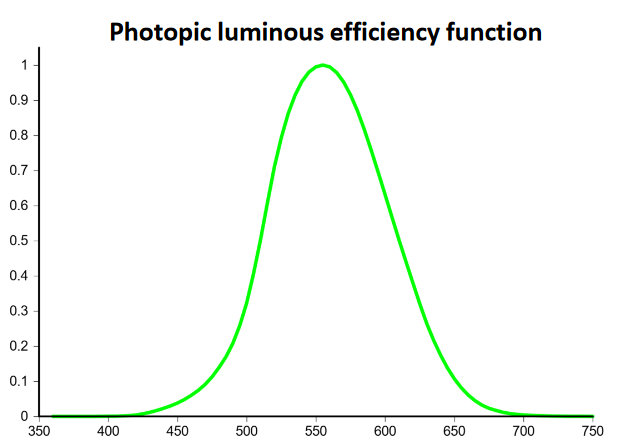
\includegraphics[width=0.5\textwidth]{immagini/funzione_fotopica}
\end{center}
Se ho una luce, per sapere come la percepisco, la moltiplico in ogni punto per la funzione
fotopica.

\section{Coefficienti tricromatici e valori RGB}
Se io dovessi regolare tre manopole, una che regola l'intenst\`a del rosso, una del verde e
una del blu e volessi ottenere una luce bianca alla fine avrei tre valori diversi per ogni
manopola, diciamo $r, g, b$. Quello che vogliamo, per\`o, \`e che il bianco, che \`e la somma
di tutti i colori, sia effettivamente rappresentato come combinazione dei tre colori (rosso,
verde e blu) ognuno col massimo valore e soprattutto vogliamo che questo valore sia uguale
per tutti e 3 i colori. Non devono perci\`o dipendere dalla nostra percezione.

Se volessi rappresentare il tutto con un'equazione sarebbe cos\`i.
\[ Bianco = r \cdot m_r \oplus g \cdot m_g \oplus b \cdot m_b \]
dove $a \oplus b$ indica la percezione delle luci $a$ e $b$ sovrapposte e dove
$m_r, m_g, m_b$ sono delle costanti che valgono
\[ m_r = 1 \quad m_g = 4.39 \quad m_b = 0.0048 \]
l'obbiettivo \`e quello di ottenere
\[ r \cdot m_r = g \cdot m_g = b \cdot m_b \]
Ecco che entrano in gioco i \textbf{coefficienti tricromatici} definiti come segue
\begin{gather*}
	\alpha = \frac{r \cdot m_r}{r \cdot m_r + g \cdot m_g + b \cdot m_b} \\
	\\
	\beta = \frac{g \cdot m_g}{r \cdot m_r + g \cdot m_g + b \cdot m_b} \\
	\\
	\gamma = \frac{b \cdot m_b}{r \cdot m_r + g \cdot m_g + b \cdot m_b}
\end{gather*}
A questo punto ho che il generico colore $C$ \`e dato da
\[ C = \alpha \oplus \beta \oplus \gamma \]
vale inoltre che
\[ \alpha + \beta + \gamma = 1 \]
Questo procedimento ha come risultato quello di non considerare la \emph{luminanza} e tenere
di conto solo la mistura di colori nella stessa misura per ogni primario.

Se volessimo invece ottenere la luminanza di un certo colore, sapendo i suoi coefficienti
tricromatici dovremmo calcolare
\[ L = \alpha \cdot m_r + \beta \cdot m_g + \gamma \cdot m_b \]

Ma come facciamo a ottenere i valori RGB di un colore non spettrale ?
Dobbiamo sapere quanto rosso, quanto verde e quanto blu mettere. La "quantit\`a" di colore che
dobbiamo mettere \`e data dalle seguenti sommatorie
\begin{gather*}
	R = \sum_{\lambda = 380}^{\lambda = 780} \overline{r}(\lambda) E(\lambda) \\
	\\
	G = \sum_{\lambda = 380}^{\lambda = 780} \overline{g}(\lambda) E(\lambda) \\
	\\
	B = \sum_{\lambda = 380}^{\lambda = 780} \overline{b}(\lambda) E(\lambda) \\
\end{gather*}
Dove le funzioni soprasegnate sono la \emph{color matching function} dello specifico colore,
ovvero quanto di quel colore vedo ad una determinata frequenza della luce, nel punto
$\lambda$ mentre $E(\lambda)$ equivale all'energia che arriva nello spettro.

\section{Spazi di colori}
Per ottenere sfumature di colore in modo pi\`u agevole sono stati introdotti
degli \textbf{spazi di colori}.

\subsection{HSV}
L'HSV (\textbf Hue, \textbf Saturation and \textbf Value) funziona in questo modo:
\begin{itemize}
	\item Il primo valore \`e la tinta, il colore scelto.
	\item Il secondo valore \`e la saturazione e l'idea \`e quella di impostare con essa,
	      quanto grigio si vuole aggiungere al colore scelto. Se la saturazione \`e
	      massima non aggiunger\`o grigio al mio colore, se \`e minima otterr\`o proprio
	      il grigio. Il valore minimo \`e 0 e il valore massimo \`e 1 ma questi valori
	      dipendono in modo proporzionale dal prossimo valore.
	\item Il terzo valore \`e la luminosit\`a del grigio che sto aggiungendo al mio colore.
	      Con il valore massimo otterr\`o il bianco, con il minimo otterr\`o il nero
	      (valore minimo 0, valore massimo 1).
\end{itemize}

\subsection{HSL}
L'HSL (\textbf Hue, \textbf Saturation and \textbf Lightness) molto simile al precedente. In
questo caso abbiamo il valore della \textbf{luminosit\`a} che va da $-0.5$ a $0.5$ in questo
caso la saturazione \`e massima con luminosit\`a 0 e si abbassa se la luminosit\`a cala o
incrementa.